\documentclass[11pt]{article}
\usepackage[a4paper,margin=25mm]{geometry}
\usepackage[T1]{fontenc}
\usepackage{lmodern,microtype,amsmath,amssymb,amsthm,graphicx,booktabs,array}
\usepackage[colorlinks=true,allcolors=blue]{hyperref}
\usepackage{fancyhdr}
\pagestyle{fancy}\fancyhf{}\fancyhead[L]{\small Division timing and daughter qualification}\fancyhead[R]{\small Theoretical methods}\fancyfoot[C]{\thepage}
\setlength{\headheight}{14pt}
\newtheorem{theorem}{Theorem}\newtheorem{proposition}[theorem]{Proposition}\newtheorem{corollary}[theorem]{Corollary}
\newcommand{\E}{\mathbb E}\newcommand{\Prb}{\mathbb P}\newcommand{\pos}[1]{\left[#1\right]_+}
\title{Division timing and daughter rematuration:\\sharp joint bounds for cardiomyocyte lineage output at a deadline}
\author{Syed Umer Hannan\\[3pt]\small Batterjee Medical College\\\small Jeddah, Saudi Arabia}\date{}
\hypersetup{pdfauthor={Syed Umer Hannan},pdftitle={Division timing and daughter rematuration: sharp joint bounds for cardiomyocyte lineage output at a deadline}}
\begin{document}\maketitle
\begin{abstract}
Verified cardiomyocyte division and later restoration of a qualifying phenotype are distinct observations. Predicting qualified daughter output at a deadline from their separate time distributions requires a dependence assumption that may be unmeasured. We formulate this problem with a shared division time and two potentially dependent daughter rematuration latencies. For finite-support marginals, we derive the complete attainable region of expected qualified output and the probability that neither daughter qualifies. A constructive proof reduces the three-variable coupling problem to a two-dimensional transport table and one nonnegative slack per division-time stratum. The resulting linear programme supplies sharp boundaries rather than a fitted lineage reconstruction. A two-stratum case gives the explicit lower bound $\Prb(Y=0)\geq[1+a-\E Y]_+$, where $a$ is the fraction of divisions early enough that every supported latency finishes before the deadline. This can be strictly stronger than the generic mean-only bound. We also construct a reversal in which both timing marginals are faster but actual deadline output is lower, and show exactly what division--daughter pairing and complete sister follow-up identify. The resulting measurement hierarchy distinguishes the information supplied by unpaired timing summaries, division--daughter pairs and complete sister follow-up. The analysis addresses lineage measurements in cardiac regeneration and is illustrated with synthetic distributions.
\end{abstract}

\section{Introduction}
A regenerative intervention can produce evidence of cardiomyocyte division without establishing how many daughter cells meet a prespecified phenotype at the intended assessment time. This distinction has a biological basis. Adult mammalian cardiomyocyte division and redifferentiation have been followed experimentally, with calcium-dependent signaling contributing to daughter-cell functional restoration \cite{wang}. In zebrafish, LRRC10 and the cardiac dyad link redifferentiation to control of proliferation, with related effects in mammalian cardiomyocytes \cite{nguyen}. In adult mouse hearts, ERBB2-associated functional recovery can coexist with residual molecular dedifferentiation \cite{shakked}. A transcriptomic maturity score, sarcomere appearance and contractile function therefore cannot be treated as interchangeable endpoints.

Separate marginals may arise when published summaries discard pairing, or when compatible random subsets of the same cohort are reported. Measuring a daughter latency generally requires knowing its local division time in the original experiment; retaining that pairing can therefore be a reporting improvement rather than a new wet-laboratory assay.

The relevant inference problem is temporal as well as phenotypic. An early division followed by slow rematuration may finish at the same time as a late division followed by rapid rematuration. Marginal distributions alone omit this pairing. Moreover, sisters share a division time, so their deadline outcomes cannot be assigned independently of that time without additional assumptions. We ask what joint combinations of mean output and zero-qualified-daughter probability are compatible with the available timing information.

Bounds for sums with unknown dependence are classical \cite{makarov}, and transport methods already appear in cardiac and lineage analyses. PILOT compares patient-level samples using optimal transport \cite{pilot}; moslin combines lineage and expression information to reconstruct temporal relationships, including fibroblast trajectories during zebrafish heart regeneration \cite{moslin}. Our task differs: we retain all admissible timing pairings and determine an endpoint identified set. We do not infer a preferred lineage map from expression similarity or assign a biologically unverified transport cost. The scalar mean bound is a standard transport problem. The central result here is its combination with conditional sister dependence into a complete joint output region, with a constructive reduction that avoids the full three-index probability array.

\section{Observable quantities and scope}
Fix one protocol, founder population and assessment deadline $T\geq0$. First condition on founders that complete exactly one verified binary division by $T$ in the prespecified attempt. Daughters do not divide again within this analysis. Let $0\leq D\leq T$ be division completion time from a common experimental origin, and $L_1,L_2\in[0,\infty]$ the daughter latencies from division to the selected qualification event. Define
\begin{equation}
 H_T(d,l)=\mathbf1\{d+l\leq T\},\qquad
 Y_T=H_T(D,L_1)+H_T(D,L_2).
 \label{eq:observable}
\end{equation}
Thus $Y_T\in\{0,1,2\}$. Zero output means neither daughter meets this endpoint; it is not synonymous with death or arrhythmia. The latency distribution includes failures as $+\infty$ when they are known to be failures, rather than silently excluding them.

If qualification is defined as first achievement, equation~\eqref{eq:observable} counts achievement by $T$, not survival thereafter. For qualification \emph{at} $T$, one can instead use a deadline-specific latency $L_j^{(T)}$: retain the first qualifying time only for daughters qualifying at $T$, and assign $+\infty$ to those not qualifying at $T$. The same fixed-deadline theorem then applies, but these marginals are deadline-specific and must not be interpreted as one invariant first-passage distribution. Unknown status from incomplete follow-up is not a known $+\infty$ outcome.

We randomly label sisters. This ensures identical daughter marginals without assuming independence or biological symmetry of permanently labelled daughters. Each binary lineage contributes two daughters, so sampling one daughter uniformly within each lineage defines the relevant marginal without variable-family-size weighting. Both marginals must describe the same protocol and conditional founder population. Combining a division distribution from one species with a latency distribution from another does not satisfy this condition.

For finite supports, write
\begin{equation}
 a_i=\Prb(D=d_i),\quad b_j=\Prb(L_1=l_j)=\Prb(L_2=l_j),\quad
 H_{ij}=\mathbf1\{d_i+l_j\leq T\}.
\end{equation}
There are $m$ division-time states and $n$ latency states, with nonnegative masses summing to one. Exact event times or a justified discrete-state model give this representation. Binning interval-censored times at their midpoints does not preserve exact deadline classification. Our implemented exact-support theorem should not be claimed as an exact continuous-time or interval-censoring result.

\section{Sharp joint region from a reduced transport problem}
Define the transport polytope
\begin{equation}
 \mathcal Z(a,b)=\left\{z_{ij}\geq0:\sum_jz_{ij}=a_i,\ \sum_i z_{ij}=b_j\right\},\qquad
 e_i(z)=\sum_jH_{ij}z_{ij}.
\end{equation}
Here $z_{ij}$ is the joint law of division time and one uniformly labelled daughter's latency. The quantity $e_i$ is the probability mass of qualification in division stratum $i$. Put
\begin{align}
 \mu_-&=2\min_{z\in\mathcal Z}\sum_i e_i(z),&
 \mu_+&=2\max_{z\in\mathcal Z}\sum_i e_i(z),\label{eq:means}\\
 \phi(\mu)&=\min_{\substack{z\in\mathcal Z\\2\sum_i e_i(z)=\mu}}
 \sum_i\pos{a_i-2e_i(z)}.\label{eq:phi}
\end{align}

\begin{theorem}[Complete deadline-output region]\label{thm:main}
Among all laws of $(D,L_1,L_2)$ with the specified division and equal daughter marginals, the attainable pairs $(\E Y_T,\Prb(Y_T=0))$ are exactly
\begin{equation}
 \mathcal S_T=\left\{(\mu,p_0):\mu_-\leq\mu\leq\mu_+,\quad
 \phi(\mu)\leq p_0\leq1-\mu/2\right\}.
 \label{eq:region}
\end{equation}
Every endpoint is attained at the specified deadline. Extremising laws may differ between deadlines; separate pointwise bounds do not assert a single law attains an entire boundary curve over time. Computing $\phi$ requires $mn+m$ nonnegative variables, rather than the $mn^2$ variables of an ordered three-marginal law.
\end{theorem}
\begin{proof}
Any admissible law may be symmetrised by swapping daughter labels with probability one half; this leaves both observables unchanged. Its single-daughter law is then some $z\in\mathcal Z$. Conditional on $D=d_i$ with $a_i>0$, each daughter qualifies with probability $e_i/a_i$. The elementary two-Bernoulli bounds imply that the unconditional mass $t_i$ of two failures in stratum $i$ satisfies
\begin{equation}
 [a_i-2e_i]_+\leq t_i\leq a_i-e_i.\label{eq:row}
\end{equation}
Summing gives $\mu=2\sum_i e_i$ and $p_0=\sum_i t_i$, establishing necessity. The image of the convex compact polytope under the linear mean functional is the entire interval $[\mu_-,\mu_+]$.

For sufficiency, choose any $z$ attaining the minimum in \eqref{eq:phi}. In each stratum assign unconditional binary-status masses
\[
 p_{00,i}=t_i,\quad p_{10,i}=p_{01,i}=a_i-e_i-t_i,\quad
 p_{11,i}=2e_i-a_i+t_i.
\]
These are nonnegative exactly on \eqref{eq:row}, sum to $a_i$, and give each daughter success mass $e_i$. Given the status pair and stratum, draw each latency from the normalised restriction of $z_{ij}$ to the corresponding success or failure set. Empty sets have zero status mass and require no draw. This constructs a full joint law with the required marginals and outcomes. By continuously moving each $t_i$ between its lower and upper endpoints, any total between $\phi(\mu)$ and $\sum_i(a_i-e_i)=1-\mu/2$ is obtained. Zero-mass strata contribute nothing. Compactness ensures all minima and maxima exist.
\end{proof}

The construction preserves the supplied marginals and establishes attainability of the entire region. The reduction combines conditional Bernoulli bounds with transport optimisation to isolate the effect of a shared division time.

\subsection{Linear programme and dual certificates}
Introduce $t_i\geq0$ and impose $t_i+2\sum_jH_{ij}z_{ij}\geq a_i$. Minimising $\sum_i t_i$ subject to these constraints, the row/column sums and $2\sum_{ij}H_{ij}z_{ij}=\mu$ gives \eqref{eq:phi}. The optimal $t_i$ never exceeds $a_i$, so the implementation may add that upper bound. The lower frontier is convex and piecewise linear on its feasible mean interval, as follows from the finite linear programme or by mixing admissible joint laws.

One exact dual form, without the redundant upper bounds on $t$, is
\begin{equation}
 \sup_{u,v,w,\lambda}\left\{\sum_i(u_i+\lambda_i)a_i+\sum_jv_jb_j+w\mu\right\},\label{eq:dual}
\end{equation}
where $u,v,w$ are unrestricted, $0\leq\lambda_i\leq1$, and
\begin{equation}
 u_i+v_j+2(\lambda_i+w)H_{ij}\leq0\quad\hbox{for all }i,j.
\end{equation}
To verify weak duality directly, multiply these inequalities by $z_{ij}$ and sum. Using the marginal and mean constraints bounds \eqref{eq:dual} above by $\sum_i\lambda_i(a_i-2e_i)\leq\sum_i[a_i-2e_i]_+$. Finite-dimensional linear-programming duality gives equality at a feasible mean. The supplied solver reports numerical primal/dual residuals; these floating-point diagnostics are not interval-arithmetic certificates. The analytical example below also has an exact certificate.

\section{A closed-form case with a stronger lower loss bound}
Consider two division states (early, late), with early mass $a$, and two latency states (fast, slow), with fast mass $b$. Suppose
\begin{equation}
 d_E+l_S\leq T,\qquad d_L+l_F\leq T<d_L+l_S,
 \quad H=\begin{pmatrix}1&1\\1&0\end{pmatrix}.\label{eq:two}
\end{equation}
Both division times can lie before the deadline. Early lineages always complete qualification; late lineages do so only with a fast latency.

\begin{corollary}[Two-stratum frontier]\label{cor:two}
The complete region is
\begin{align}
 2\max(a,b)&\leq\mu\leq2\min(1,a+b),\\
 [1+a-\mu]_+&\leq p_0\leq1-\mu/2.\label{eq:twobound}
\end{align}
\end{corollary}
\begin{proof}
Let $x=z_{L,F}$. Transport feasibility gives $\max(0,b-a)\leq x\leq\min(b,1-a)$. The success masses are $e_E=a$ and $e_L=x$, hence $\mu=2(a+x)$ and $\phi=[1-a-2x]_+=[1+a-\mu]_+$. Theorem~\ref{thm:main} proves attainability of the full interval. Alternatively, early lineages always contribute two successes, so $p_2\geq a$. The identity $p_0=1-\mu+p_2$ gives the strengthened lower bound directly. In the dual, $w=-1$, $\lambda_E=0$, $\lambda_L=1$, $u_E=2$, $u_L=0$ and both $v_j=0$ certify $1+a-\mu$ exactly; the zero dual certifies zero.
\end{proof}

For hypothetical $a=b=1/2$ and $\mu=1.2$, the sharp zero-output interval is $[0.3,0.4]$. A mean-only analysis permits $[0,0.4]$ and would fail to exclude the impossible pair $(1.2,0.1)$. This is not a prediction that 30\% of real cardiac lineages fail. It is a testable incompatibility statement for the specified timing marginals and endpoint. More generally, combining a measured mean with a measured zero-output fraction outside \eqref{eq:region} shows that at least one supplied marginal, classification, sampling-population assumption or observation is incompatible; it does not identify which one is wrong.

\begin{figure}[htbp]\centering
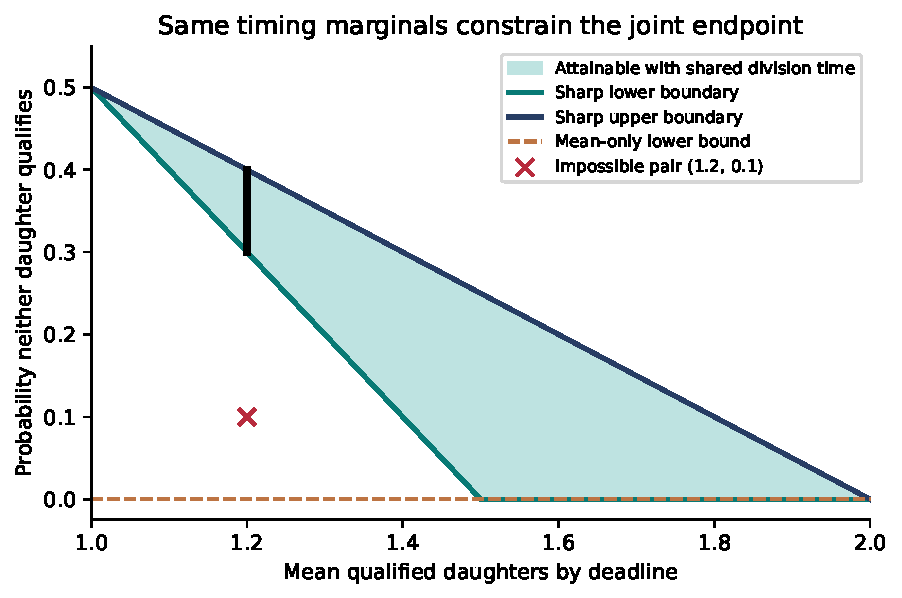
\includegraphics[width=.9\linewidth]{../figures/frontier.pdf}
\caption{Exact synthetic two-stratum region with $a=b=1/2$. At mean 1.2 the allowed zero-output probability is 0.3--0.4. The crossed point passes the generic mean-only restriction but violates the shared-timing constraint.}
\end{figure}

\section{Why faster marginal times do not rank actual protocols}
A second exact example separates marginal improvement from paired completion. Set $T=2.5$. In protocol A, both $D$ and $L$ have masses one half at 0 and 2. Pair early division with fast latency and late division with slow latency; set sister latencies equal. One half of lineages finish at time 0 and one half at time 4, so $\E Y_T=1$ and $p_0=1/2$.

In protocol B, both marginals instead have masses one half at 0.2 and 2.2. Pair early division with slow latency and late division with fast latency, again with equal sisters. All lineages finish at 2.4, giving $\E Y_T=2$ and $p_0=0$. Each marginal of A is stochastically faster than its counterpart in B, yet A has lower actual deadline output. Arbitrary dependence differs between protocols. This does not contradict monotonicity when individual paired times improve, or claim that such a reversal occurs biologically. It proves that marginal speed alone is insufficient for that conclusion. The example persists over an open range of deadlines and small positive time shifts; zero latency is permitted but is not essential to the reversal.

\begin{figure}[htbp]\centering
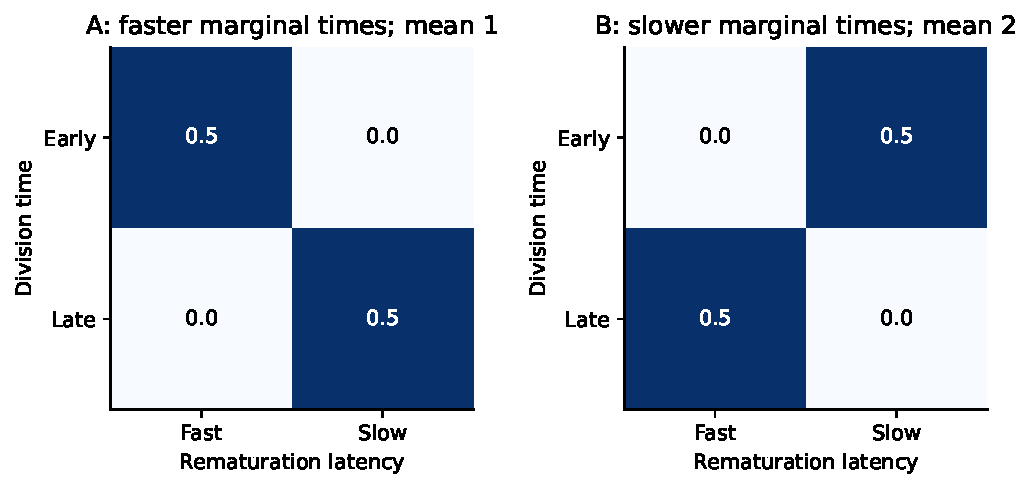
\includegraphics[width=\linewidth]{../figures/ranking.pdf}
\caption{Synthetic division--latency transport tables for the ranking reversal. Entries are probabilities. Both marginal time distributions are faster in A, but the cross-pairing in B concentrates all completion times before the shared deadline. Sisters are perfectly coupled in both constructions.}
\end{figure}

\section{What additional measurements identify}
If division time and one randomly chosen daughter's latency are observed jointly, the table $z$ is known. Then the mean is identified as $2\sum_i e_i$ and the zero-output probability lies in
\begin{equation}
 \sum_i[a_i-2e_i]_+\leq p_0\leq1-\sum_i e_i.\label{eq:paired}
\end{equation}
This is an immediate sharp consequence of the constructive proof. Full latency distributions within strata are unnecessary for these two observables once the stratum masses $a_i$ and qualified single-daughter masses $e_i$ are known. Measuring both sisters at the same deadline identifies $p_0$ directly. These are population-identification statements; finite samples retain sampling uncertainty.

\begin{center}\small
\begin{tabular}{p{.32\linewidth}p{.27\linewidth}p{.29\linewidth}}\toprule
Available information & Mean output & Zero-output probability\\\midrule
Separate division and daughter-latency marginals & Interval from transport & Joint region in Theorem 1\\
Division paired to one random daughter & Identified & Sharp interval in \eqref{eq:paired}\\
Division paired to both daughters & Identified & Identified\\\bottomrule
\end{tabular}
\end{center}

For an unconditioned activated-founder population, let $q$ be the proportion that divided by $T$ in the defined one-attempt cohort and $r_T$ qualification probability of nondividing founders at $T$. Then
\begin{equation}
 \E Y_T^{\mathrm{all}}=(1-q)r_T+q\mu,\qquad
 \Prb(Y_T^{\mathrm{all}}=0)=(1-q)(1-r_T)+qp_0.\label{eq:affine}
\end{equation}
Founders that will divide only after $T$ belong to the nondividing-at-$T$ branch, so their current qualification is not lost from the count. The whole region transforms affinely. When $q=0$ the divided-lineage problem is irrelevant. This extension preserves nondividing recovery without assuming a feasible intervention changes only $q$. Comparing protocols requires their own compatible marginals and branch definitions.

\section{Biological applicability and measurement boundaries}
The intended use is an inference audit of a defined regeneration experiment: are claimed deadline mean output and zero-output frequency jointly compatible with observed division and daughter-qualification timing? A second use is deciding whether to retain division--daughter and sister pairing information. These uses follow from the theorem and do not require a calibrated model of ventricular mechanics.

There is evidence that the proposed observables are experimentally meaningful, but no single universal maturation latency. Wang et al. followed adult mammalian cardiomyocyte dedifferentiation, division and redifferentiation \cite{wang}. Shakked et al. separated recovery of function from persistent molecular signatures after ERBB2 induction \cite{shakked}. Nguyen et al. linked redifferentiation to calcium-handling structures and LRRC10 \cite{nguyen}. More recently, Bouhamida et al. used time-lapse microscopy to observe completed cytokinesis in adult human cardiomyocytes and assessed sarcomere integrity and calcium mobilization \cite{human}. The latter also cautions against imposing an obligatory long period of complete sarcomere loss on every division. Our model allows zero latency and does not equate dedifferentiation with an invariant functional deficit.

These studies support endpoint selection and the measurement architecture; they do not provide calibration for our synthetic examples. In particular, a tissue echocardiographic recovery curve is not a distribution of individual daughter latencies. Separate functional assays do not automatically preserve the lineage pairing needed here. Selected published movies cannot be treated as an unbiased sample of all divisions or failures. We did not assert that the reviewed sources contain a complete, suitable joint dataset.

A concrete data record would retain donor or animal identifier, protocol, founder and daughter identifiers, the common experimental origin, verified cytokinesis time, qualification criterion, first qualification time if observed, deadline status, last observation time and censoring reason. Structural and functional criteria should be analysed separately or combined by a prespecified rule. Missing cells cannot be silently removed from the denominator. Transcriptomic pseudotime cannot be substituted for elapsed time without a separate validated mapping. Tissue-level function, arrhythmia, repeat division and spatial interactions remain outside this one-attempt endpoint.

\subsection{Sampling uncertainty and censoring}
The theorem assumes population marginals, not estimated marginals without error. A confidence region $\mathcal C$ for compatible marginals can be propagated by taking the union of the identified sets over $\mathcal C$. If the true marginals lie in $\mathcal C$ with probability at least $1-\alpha$, the resulting union contains the true endpoint pair with at least that probability, by set inclusion. This observation does not supply a valid confidence region by itself. Dependence within donors or animals must be represented in the sampling design; cells are not automatically independent replicates.

Right-censored qualification times require a set of possible marginals or a justified censoring model. Setting all censored values to $+\infty$ generally treats an unresolved observation as failure and is inappropriate. Conversely, discarding them conditions on observation and can bias the marginal. The provided solver accepts exact discrete marginals and makes neither adjustment automatically. It is a verified theoretical implementation, not a complete inference pipeline for uncurated movies.

\section{Numerical verification}
The implementation passes six test methods. Across 200 pseudorandom binary masks with one to four states per dimension, the reduced lower and upper boundaries were compared with an independently assembled three-marginal linear programme at the lower endpoint, midpoint and upper endpoint (including repeated means in degenerate cases): 1,200 objective comparisons. The constructive lift was checked at lower, upper and intermediate row couplings, giving 1,800 full-law checks. These verify both daughter marginals, division marginals, mean, zero-output probability and nonnegative masses to numerical tolerances. The tests include non-monotone binary masks because the reduction itself only uses binary qualification, not the ordering of times.

A separate two-stratum grid contains 81 marginal pairs and five feasible means each, giving 405 comparisons with the closed-form result. Further checks cover deadline equality, a known failure atom, empty mean slices, invalid inputs and the ranking reversal. The displayed frontier contains 101 mean values with primal and dual diagnostics. All numerical checks run on an ordinary CPU.

The shared division-time formulation yields a joint endpoint region and an explicit measurement hierarchy. Its ingredients---fixed-marginal bounds, conditional Bernoulli bounds and linear-programming duality---are established methods. The present analysis concerns exact finite-support marginals. Empirical use requires compatible measurements and appropriate treatment of censoring and sampling uncertainty.

\section{Conclusion}
At a fixed assessment time, division and daughter rematuration cannot generally be combined from separate marginals into a unique regenerative-output prediction. The shared division time creates joint endpoint restrictions that a mean-only calculation can miss. A reduced transport problem yields the complete sharp region and constructive witnesses. Pairing division with one daughter identifies the mean; tracking both sisters additionally identifies lineage-level zero output. This provides a mathematically explicit measurement strategy for cardiac regeneration studies while keeping biological validation distinct from theorem verification.

\section*{Data and code availability}
All numerical examples use hypothetical parameters. Source code, tests, constructed joint-distribution witnesses, result tables and figures are provided in the accompanying package. No newly collected human or animal data are analysed. The reproduction script regenerates the reported numerical results and runs the verification suite.

\begin{thebibliography}{99}
\bibitem{wang} Wang WE, Li L, Xia X, et al. Dedifferentiation, proliferation, and redifferentiation of adult mammalian cardiomyocytes after ischemic injury. \emph{Circulation}. 2017;136:834--848. \href{https://doi.org/10.1161/CIRCULATIONAHA.116.024307}{doi:10.1161/CIRCULATIONAHA.116.024307}.
\bibitem{nguyen} Nguyen PD, Gooijers I, Campostrini G, et al. Interplay between calcium and sarcomeres directs cardiomyocyte maturation during regeneration. \emph{Science}. 2023;380:758--764. \href{https://doi.org/10.1126/science.abo6718}{doi:10.1126/science.abo6718}.
\bibitem{shakked} Shakked A, Petrover Z, Aharonov A, et al. Redifferentiated cardiomyocytes retain residual dedifferentiation signatures and are protected against ischemic injury. \emph{Nature Cardiovascular Research}. 2023;2:383--398. \href{https://doi.org/10.1038/s44161-023-00250-w}{doi:10.1038/s44161-023-00250-w}.
\bibitem{human} Bouhamida E, Vadakke-Madathil S, Mathiyalagan P, et al. Cyclin A2 induces cytokinesis in human adult cardiomyocytes and drives reprogramming in mice. \emph{npj Regenerative Medicine}. 2025;10:47. \href{https://doi.org/10.1038/s41536-025-00438-7}{doi:10.1038/s41536-025-00438-7}.
\bibitem{makarov} Makarov GD. Estimates for the distribution function of a sum of two random variables when the marginal distributions are fixed. \emph{Theory of Probability and Its Applications}. 1982;26(4):803--806. \href{https://doi.org/10.1137/1126086}{doi:10.1137/1126086}.
\bibitem{pilot} Joodaki M, Shaigan M, Parra V, et al. Detection of PatIent-Level distances from single cell genomics and pathomics data with Optimal Transport (PILOT). \emph{Molecular Systems Biology}. 2024;20:1 (online December 2023). \href{https://doi.org/10.1038/s44320-023-00003-8}{doi:10.1038/s44320-023-00003-8}.
\bibitem{moslin} Lange M, Piran Z, Klein M, et al. Mapping lineage-traced cells across time points with moslin. \emph{Genome Biology}. 2024;25:277. \href{https://doi.org/10.1186/s13059-024-03422-4}{doi:10.1186/s13059-024-03422-4}.
\end{thebibliography}
\end{document}
